\section{Rappels sur la programmation orientée objet}
\subsection{Quelques définitions}

La programmation orientée objet est une technique de programmation qui consiste à découper un programme en plusieurs objets qui interagissent entre eux. 
Chaque objet est une instance d'une classe. Une classe est un ensemble d'attributs et de méthodes. Les attributs sont des variables propres à chaque objet. Les méthodes sont des fonctions propres à chaque objet.

%%%% Idée %%%%
Il s'agit d'une façon de penser la programmation. Si elle peut paraître plus complexe au début, elle permet de structurer le code, de le rendre plus lisible et plus facilement modifiable. 

La définition des objets (création de classes) peut être complexe, mais l'utilisation des objets est largement simplifiée. C'est d'ailleurs un avantage majeur de la programmation orientée objet : l'utilisateur d'un objet n'a pas besoin de connaître sa définition pour l'utiliser. Il lui suffit de connaître les méthodes et les attributs de l'objet.

%%%% /Idée %%%%

%%%% Explication %%%%
Un objet est une instance d'une classe. Cela veut simplement dire qu'une classe définit une structure (attributs et méthodes) et qu'un objet est un cas particulier de cette structure. Par analogie, on peut parler des plans d'une maison qui définissent ce qu'est une maison (nombre de pièces, surface, etc.) et des maisons qui sont des instances de ces plans. 

Chaque maison pourra avoir un nombre de pièces différentes, une couleur de toit différente, mais toutes les maisons auront les mêmes caractéristiques de base (elles auront toutes un toit, des pièces, des murs, des fenêtres, etc.).

\begin{center}
    %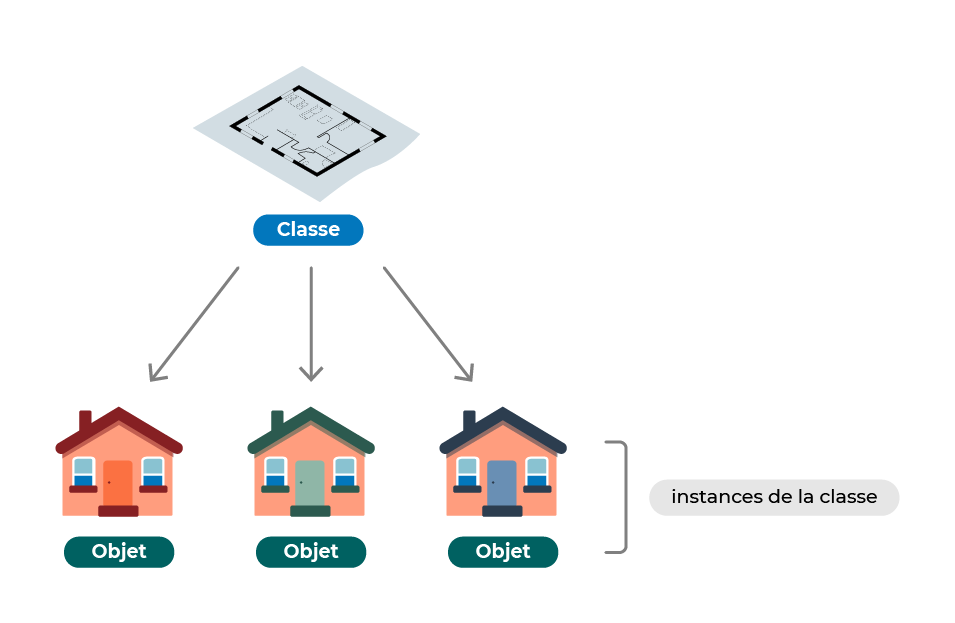
\includegraphics[width=.8\textwidth]{classe_exemplePlanMaison.png} 
\end{center}


D'un point de vue extérieur, un objet est une "boite noire" dont les détails d'implémentation sont cachés. On ne peut pas savoir comment est codé un objet, on intéragit avec lui par l'intermédiaires des fonctions d'interfaces. C'est le principe d'encapsulation.

\begin{UPSTIinfor}{Principe d'encapsulation}
    L'encapsulation est un principe de la programmation orientée objet qui consiste à cacher les détails d'implémentation d'un objet. L'accès aux données de l'objet ne peut alors se faire que par l'intermédiare des services proposées. 

    Cela a pour objectif d'en simplifier l'utilisation mais également de \textbf{garantir l'intégrité des données} contenues dans l'objet. En effet, les fonctions d'interfaces mises en places contrôlent la bonne utilisation des données.
\end{UPSTIinfor}

\UPSTIexemple[Etape d'un grafcet]{
    On peut définir une classe \emph{CStep} qui représente une étape d'un grafcet. Cette classe peut contenir, entre autres, les attributs et méthodes suivants :

    \begin{minipage}{.5\linewidth}
        \paragraph{Attributs}
            \begin{itemize}
                \item \textbf{m\_name} : nom de l'étape
                \item \textbf{m\_xActivityBit} : bit d'activité (actif ou non)
                \item \textbf{m\_tActivationDuration} : temps d'activation de l'étape
            \end{itemize}
    \end{minipage}%
    \begin{minipage}{.5\linewidth}
        \paragraph{Méthodes}
            \begin{itemize}
                \item \textbf{MInit} : Initialise l'étape
                \item \textbf{MActivate} : active l'étape
                \item \textbf{MDeactivate} : désactive l'étape
            \end{itemize}
    \end{minipage}
    Chaque étape du grafcet sera alors un objet de la classe \emph{CStep}.
}

\begin{UPSTIinfor}{La notion d'Héritage}
    L'héritage est un principe de la programmation orientée objet qui consiste à créer une nouvelle classe à partir d'une classe existante. La nouvelle classe \textbf{hérite} alors des attributs et méthodes de la classe existante. 

    Par exemple, on peut créer une classe \emph{Forme} qui contient les attributs et méthodes communs à toutes les formes géométriques fermées (comme son aire). On peut ensuite créer une classe \emph{Rectangle} qui hérite de la classe \emph{Forme} et qui contient, en plus, les attributs et méthodes spécifiques aux rectangles. On peut ensuite créer une classe \emph{Cercle} qui hérite de la classe \emph{Forme} et qui contient les attributs et méthodes spécifiques aux cercles.
\end{UPSTIinfor}

\begin{UPSTIinfor}{Le Polymorphisme}
    Le polymorphisme est un principe de la programmation orientée objet qui consiste à utiliser un objet de manière différente en fonction du contexte. 

    Plus spécifiquement, le polymorphisme autorise à utiliser un même nom pour des méthodes différentes selon si elle s'applique sur un contexte ou un autre. 

    En reprenant l'exemple précédent, on peut créer une méthode \emph{MComputeArea} dans la classe \emph{Forme} qui calcule l'aire de la forme. Cette méthode sera différente dans la classe \emph{Rectangle} et dans la classe \emph{Cercle} car l'aire d'un rectangle et l'aire d'un cercle ne se calculent pas de la même manière. En fonction de l'objet utilisé, la méthode \emph{MComputeArea} sera différente.
\end{UPSTIinfor}

%%% TODO : Ajouter la notion d'interface %%%